\section{Comunicazione Java Prolog}
\label{java-prolog}
\subsection{JPL Library}
\nocite{swi:jpl}
La libreria utilizzata per permettere la bidirezionalità della comunicazione tra Java e Prolog, è stata la \emph{JPL 3.1.4 alpha}\footnote{Scaricabile da \url{http://mvnrepository.com/artifact/jpl/jpl/3.1.4-alpha}} (\textbf{J}ava-calls-\textbf{P}rolog \textbf{L}ibrary)

Le API messe a disposizione dalla libreria JPL permettono la creazione di oggetti Java che andranno a inglobare gli elementi che saranno poi utilizzati lato Prolog. La struttura gerarchica delle classi presenti nella libreria è la seguente:
\begin{Verbatim}
Term
|
+--- Variable
|
+--- Compound
|      |
|      +--- Atom
|
+--- Integer
|
+--- Float

Query

JPLException
|
+-- PrologException
\end{Verbatim}

Le classi Term-based sono in grado di adattare al meglio la concreta sintassi strutturata dei termini di Prolog, in quanto non esiste una corrispondenza diretta con un particolare termine di Prolog; piuttosto, esistono diversi significati assunti dalla classe Term, si va dalla necessità di creare delle strutture da essere utilizzate all'interno di query Prolog, fino ad arrivare al tipo di rappresentazione, con relativa esplorazione, dei risultati ottenuti dalla query.
Per astrarre quindi il concetto di termine, la classe \emph{Term} è una classe astratta istanziata da una delle sue cinque possibili sottoclassi:
\paragraph{Compounds}
Un Compound è un Termine che contiene un nome e una sequenza di argomenti di tipo Term.

\begin{javacode}
	Compound teacher_of = new Compound("teacher_of",
	new Term[] {
		new Atom("aristotle"),
		new Atom("alexander")
	}
	);
\end{javacode}

In questo esempio, la variabile java \emph{teacher\_of} si riferisce a una istanza di tipo \emph{Compound} che rappresenta il termine prolog.

\begin{prologcode}
	teacher_of(aristotle,alexander).
\end{prologcode}

\paragraph{Atom}
Un Atom è una specializzazione di \emph{Compound} avente zero parametri, il che vorrà dire che Atom sarà un Term contenente solo un nome.

\begin{javacode}
	Atom aristotle = new Atom("aristotle");
	Atom alexander = new Atom("alexander");
\end{javacode}

\paragraph{Variable}
Le Variabili sono dei Term aventi un nome identificativo il quale deve soddisfare la sintassi Prolog.

\begin{javacode}
	Variable X = new Variable("X");  //  variabile X
	Variable X = new Variable("_");  //  variabile "anonima"
	Variable X = new Variable("_Y"); // variabile Y di cui non si vuole 
	// conoscere il contenuto
\end{javacode}

\paragraph{Integer}
Un Integer è una specializzazione di \emph{Term} che mantiene la valorizzazione di tipo long di Java. Questa classe corrisponde al tipo integer di Prolog.

\begin{javacode}
	jpl.Integer i = new jpl.Integer(5);
\end{javacode}

\paragraph{Floats}
Un Float è una specializzazione di \emph{Term} che mantiene la valorizzazione di tipo double di Java. Questa classe corrisponde al tipo float di Prolog sulla quale possono essere eseguite le operazioni aritmetiche.

\begin{javacode}
	jpl.Float f = new jpl.Float(3.14159265);
\end{javacode}

\paragraph{Queries}
Ogni istanza di Query contiene un \emph{Term}, il quale rappresenta il goal da dimostrare.

\begin{javacode}
	Term goal = new Compound("teacher_of",
	new Term[] {
		new Atom("aristotle"),
		new Atom("alexander")
	}
	);
	Query q = new Query( goal );
\end{javacode}

La query q in questo esempio rappresenta la query Prolog:

\begin{prologcode}
	?- teacher_of(aristotle,alexander).
\end{prologcode}

\subsubsection{Funzionamento}
Per garantire l'interazione tra Java e Prolog, le principali istruzioni utilizzate per permettere questa comunicazione, sono state le seguenti:

\begin{javacode}
	JPL.setNativeLibraryDir("/usr/local/lib/Yap");
	prolog.consult(new Atom("prolog/main.pl"));
	prolog.retractAll("domanda", 1);
	Term toAssert = new Compound("domanda", 
	new Term[]{
		Util.textToTerm("\"" + textPane.getText() + "\"")}
	);
	prolog.asserta(toAssert);
	java.util.Hashtable<String, Term>[] hashtables = null;
	hashtables = prolog.allSolutions(new Compound("nextTag", 
	new Term[]{
		new Variable("Tag")})
	);  
\end{javacode}
\paragraph{inizialize}
I primi comandi hanno il compito di inizializzare il motore Prolog definendo 
\begin{itemize}
	\item Quali librerie utilizzare per la dimostrazione del goal (in questo caso si è deciso di utilizzare le librerie di \emph{Yap});
	\item Definire la base di conoscenza tramite i consult, i retract e gli assert, sia dei fatti che delle regole da utilizzare.
\end{itemize}
Il codice java atto a realizzare sia la consult che la retract è il seguente:

\begin{javacode}
	public boolean consult(Atom atom) {
		Term t = new Compound("consult", new Term[]{atom});
		Query query = new Query(t);
		System.out.print("[Prolog] consult: " + t + " ");
		System.out.println(query.hasSolution() ? "succeeded" : "failed");
		return query.hasSolution();
	}
\end{javacode}

\begin{javacode} 
	public void retractAll(String predicate, int arity) {  
		Term[] args = new Term[arity];
		for (int i = 0; i < args.length; i++)
		args[i] = new Variable("_");
		Term[] termToRetract = new Term[]{ new Compound(predicate, args) };    
		Term t = new Compound("retractall", termToRetract);
		Query query = new Query(t);
		System.err.print("[Prolog] retract( " + predicate + " ) ");
		System.err.println(query.hasSolution() ? "succeeded" : "failed");
	}
\end{javacode}

\paragraph{Queries}
Una volta ultimata l'inizializzazione, il passo successivo sarà quello di estrarre i risultati del tag che il sistema ha prodotto; per fare ciò, verranno create delle query parametrizzate adeguatamente da Termini e i risultati verranno inseriti all'interno di un array di tipo Hashtable.

\begin{javacode}
	public java.util.Hashtable[] allSolutions(Term t) {
		Query query = new Query(t);
		System.err.print("[Prolog] query: " + t + " ");
		System.err.println(query.hasSolution() ? "succeeded" : "failed");
		return query.allSolutions();
	}
\end{javacode}

\section{Interazione con l'utente}
\subsection{Java}
Il sistema presenta un'interfaccia grafica scritta in java, in grado di permettere l'interazione con il core del sistema scritto in Prolog, dando cosi la possibilità a qualunque tipo di stakeholders del sistema di utilizzarlo senza la necessità di dover interagire con il terminale, rendendo cosi le informazioni più leggibili e usabili; Oltre a questo, la creazione dell'interfaccia permette anche di evitare possibili errori dattilografici che si potrebbero avere in caso di interazione con il terminale.

La schermata principale dell'interfaccia sarà la seguente:
\begin{figure}[H]
	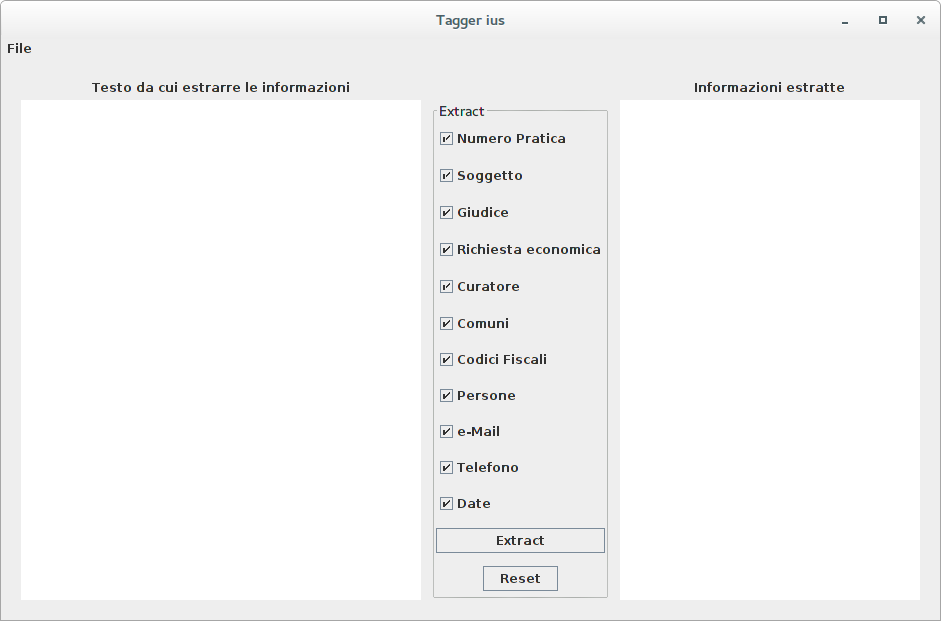
\includegraphics[width=1\textwidth]{img/interfaces/java-main.png}
	\caption{Main interfaccia grafica}
	\label{java-main}
\end{figure}

Come si può vedere, l'interfaccia minimalista permette al sistema di essere facilmente usabile infatti presenta essenzialmente tre componenti principali:
\begin{itemize}
  \item Sezione di inserimento del documento da cui si devono estrarre le informazioni;
  \item Sezione di scelta delle informazioni da estrarre;
  \item Sezione di visualizzazione dei risultati ottenuti.
\end{itemize}

Inoltre è presente anche una barra di menù dalla quale viene data la possibilità di scegliere quale motore utilizzare per la comunicazione tra java e prolog tra quelli descritti in \ref{java-prolog}:
\begin{figure}[H]
	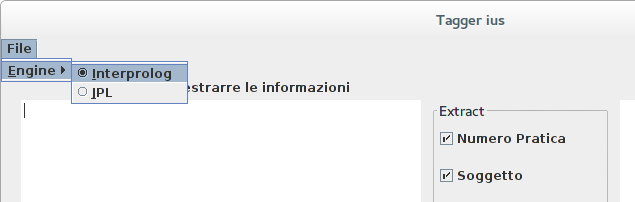
\includegraphics[width=1\textwidth]{img/interfaces/java-engine.png}
	\caption{Scelta engine java - prolog}
	\label{java-engine}
\end{figure}
\subsubsection{Sezioni ed operazioni disponibili}
    \paragraph{Inserimento}
    \label{Inserimento}
    In questa sezione viene data la possibilità di inserire il documento testuale da cui si vogliono estrarre le informazioni; con questa operazione non si fa altro che asserire un documento da dover poi essere processato dal core prolog del sistema.
    \paragraph{Scelta dei tag}
    \label{ChoiceTag}
    In questa sezione si da la possibilità all'utente di filtrare i tag da voler estrarre dal documento attraverso la selezione/deselezione della checkbox corrispondente al tag; con questa operazione si vanno a selezionare quali saranno i tag che il core prolog deve etichettare nel documento.
    \paragraph{Visualizzazione}
    \label{Visualization}
    In questa schermata invece verranno mostrate le informazioni che l'utente ha deciso di estrarre dal documento;
    \paragraph{Reset delle condizioni iniziali}
    Tramite il pulsante \emph{Reset} si ripristineranno le condizioni iniziali del sistema. In particolare, viene ripristinato lo stato iniziale:
    \begin{itemize}
      \item \emph{Interfaccia} : cancellando sia le textbox contenenti il documento inserito \ref{Inserimento} e i tag etichettati dal testo \ref{Visualization}, sia le scelte dei tag da effettuare \ref{ChoiceTag}.
      \item \emph{Core Prolog} : ritrattando il documento appena inserito nella sezione \ref{Inserimento}, riportando il sistema allo stato di partenza.
    \end{itemize}
	\subsubsection{Esempio di interazione}
	Supponiamo di voler taggare il seguente documento:
	\small
	\begin{verbatim}
	                DOMANDA DI AMMISSIONE ALLO STATO PASSIVO
                    TRIBUNALE CIVILE DI Civitavecchia
                            SEZIONE FALLIMENTARE
Procedura n. 49/2011
GIUDICE DELEGATO -  Altobello Nicola
CURATORE - Torelli Mario
                   
                   DOMANDA DI AMMISSIONE AL PASSIVO

Ill.mo signor Giudice Delegato alla procedura sopra indicata, 
il sottoscritto Simone Christian nato a Lecce il 15 luglio 1974 
con sede in Lecce C.F. QCNPLA88M04C983K domiciliato in Foggia in 
via Roma, 12 il quale dichiare di voler ricevere comunicazioni 
e notifiche a mezzo fax al seguente n. 3475459798 oppure per email 
al seguente indirizzo c.simone@libero.it

                                     CHIEDE

di essere ammesso allo stato passivo della procedure in epigrafe indicata:

in via chirografaria per 1890 dollari 
Precisando che il proprio credito deriva da prestazioni di lavoro 
subordinato in qualità di operaio.

Si allegano 2 documenti:
fattura n. 1
fattura n. 2

in via privilegiata per euro 2000 
Precisando che il proprio credito deriva da acquisto materiale.

Si allegano 2 documenti:
fattura n. 1
fattura n. 2

Civitavecchia, li 15 settembre 2013
                                                    Simone Christian
	\end{verbatim}

\subsection{Bash}
L’interazione avviene principalmente tramite l'interfaccia grafica descritta nella sezione precedente ma viene data anche la possibilità di interagire con il sistema anche senza l'ausilio di tale interfaccia, utilizzando direttamente l'interprete Prolog da terminale, previa consultazione del modulo principale del sistema denominato \emph{main.pl}; le funzionalità del sistema sono indipendenti dal metodo con cui si vuole interagire con il sistema.

\subsection{Presentazione dei risultati}

\subsection{Utilizzo della funzione spiega ragionamento}
